\documentclass[12pt]{article}
\usepackage[utf8]{inputenc}

\usepackage{lmodern}

\usepackage{enumitem}
\usepackage[margin=2cm]{geometry}

\usepackage{amsmath, amsfonts, amssymb}
\usepackage{graphicx}
%\usepackage{subfigure}
\usepackage{tikz}
\usepackage{pgfplots}
\usepackage{multicol}

\usepackage{comment}
\usepackage{url}
\usepackage{calc}
\usepackage{subcaption}
\usepackage[indent=0pt]{parskip}
\usepackage{animate}

\usepackage{array}
\usepackage{blkarray,booktabs, bigstrut}
\usepackage{bigints}

\pgfplotsset{compat=1.16}

% MATH commands
\newcommand{\ga}{\left\langle}
\newcommand{\da}{\right\rangle}
\newcommand{\oa}{\left\lbrace}
\newcommand{\fa}{\right\rbrace}
\newcommand{\oc}{\left[}
\newcommand{\fc}{\right]}
\newcommand{\op}{\left(}
\newcommand{\fp}{\right)}

\newcommand{\bi}{\mathbf{i}}
\newcommand{\bj}{\mathbf{j}}
\newcommand{\bk}{\mathbf{k}}
\newcommand{\bF}{\mathbf{F}}

\newcommand{\mR}{\mathbb{R}}

\newcommand{\ra}{\rightarrow}
\newcommand{\Ra}{\Rightarrow}

\newcommand{\sech}{\mathrm{sech}\,}
\newcommand{\csch}{\mathrm{csch}\,}
\newcommand{\curl}{\mathrm{curl}\,}
\newcommand{\dive}{\mathrm{div}\,}

\newcommand{\ve}{\varepsilon}
\newcommand{\spc}{\vspace*{0.5cm}}

\DeclareMathOperator{\Ran}{Ran}
\DeclareMathOperator{\Dom}{Dom}

\newcommand{\exo}[1]{\noindent\textcolor{red}{\fbox{\textbf{Problem {#1}}}\hrulefill}\\}
\newcommand{\qu}[4]{\noindent\textcolor{#4}{\fbox{\textbf{Section {#1} | Problem {#2}}} \hrulefill{{\fbox{\textbf{{#3} Points}}}}\\}}

\newcommand{\semester}{Spring 2023}

\newcommand{\CVup}{%

\begin{tikzpicture}
\draw[black, <->, >=latex] (-0.33, 0.5) .. controls (-0.125, 0) and (0.125, 0) .. (0.33, 0.5);
\end{tikzpicture}}

\newcommand{\CVupInc}{%
\begin{tikzpicture}
\draw[black, ->, >=latex] (0,0) .. controls (0.2, 0) and (0.4, 0.2) .. (0.5, 0.5);
\end{tikzpicture}}

\newcommand{\CVupDec}{%
\begin{tikzpicture}[rotate=270]
\draw[black, ->, >=latex] (0,0) .. controls (0.2, 0) and (0.4, 0.2) .. (0.5, 0.5);
\end{tikzpicture}}

\newcommand{\CVdown}{%
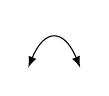
\begin{tikzpicture}
\draw[black, <->, >=latex] (-0.33, -0.5) .. controls (-0.125, 0) and (0.125, 0) .. (0.33, -0.5);
\end{tikzpicture}}

\newcommand{\CVdownInc}{%
\begin{tikzpicture}
\draw[black, ->, >=latex] (-0.5, -0.5) .. controls (-0.5, -0.3) and (-0.5, -0.1) .. (0,0);
\end{tikzpicture}}

\newcommand{\CVdownDec}{%
\begin{tikzpicture}[rotate=-90]
\draw[black, ->, >=latex] (-0.5, -0.5) .. controls (-0.5, -0.3) and (-0.5, -0.1) .. (0,0);
\end{tikzpicture}}

\begin{document}
	\noindent \hrulefill \\
	MATH-241 \hfill Pierre-Olivier Paris{\'e}\\
	Solutions Section 2-2 \hfill \semester \\\vspace*{-1cm}
	
	\noindent\hrulefill
	
	\spc
	
	\exo{12}
	\\
	That $t = 0$, the slope of the tangent line is positive and quite small. When we move towards $t = 5$, the slope increases and attain a maximum around $t = 6$. Then the slope decreases as we more towards $t = 10$. The slope becomes really small (close to zero) when we reach $t = 15$. The graph show look like this:
	
	\spc
	
	\exo{20}
	\\
	Using the definition, we have
		\begin{align*}
		f' (x) = \lim_{h \ra 0} \frac{f (x + h) - f(x)}{h} &= \lim_{h \ra 0} \frac{m (x + h) + b - (mx + b)}{h} \\
		&= \lim_{h \ra 0} \frac{mx + mh + b - mx - b}{h} \\
		&= \lim_{h \ra 0} \frac{mh}{h} = m .
		\end{align*}
	Therefore, $f'(x)$ exists for any $x$ and $f'(x) = m$.
	
	\spc
	
	\exo{25}
	\\
	The domain of the function is $(-\infty, 9]$. The derivative at $x$ is
		\begin{align*}
		f'(x) = \lim_{h \ra 0} \frac{\sqrt{9 - x -h} - \sqrt{9 - x}}{h} &= \lim_{h \ra 0} \frac{9 - x - h - 9 + x}{h (\sqrt{9 - x - h} + \sqrt{9 - x}} \\
		&= \lim_{h \ra 0} -\frac{1}{\sqrt{9 - x- h} + \sqrt{9 -x}} \\
		&= -\frac{1}{2 \sqrt{9 - x}} .
		\end{align*}
	So $f'(x) = -1/2\sqrt{9 - x}$ and the domain of $f'$ is $(-\infty , 9 )$.
	
	\spc
	
	\exo{26}
	\\
	By definition, we have 
		\begin{align*}
		f'(x) = \lim_{h \ra 0} \frac{f(x + h) - f(x)}{h} .
		\end{align*}
	Let's simplify the difference quotient:
		\begin{align*}
		\frac{f(x + h) - f(x)}{h} &= \frac{\frac{(x + h)^2 - 1}{2 (x + h) - 3} - \frac{x^2-1}{2x - 3}}{h (2x-3)(2x + 2h - 3)} \\
		&= \frac{(x^2 + 2xh + h^2 - 1)(2x - 3) - (x^2 - 1)(2x + 2h - 3)}{h (2x-3)(2x + 2h - 3)} \\
		&= \frac{(x^2 - 1) (2x - 3) + (2xh + h^2) (2x - 3) - (x^2 - 1) (2x - 3) - 2h (x^2 - 1)}{h (2x-3)(2x + 2h - 3)} \\
		&= \frac{4x^2 h - 6xh + 2xh^2 - 3h^2 - 2x^2h + 2h}{h (2x-3)(2x + 2h - 3)} \\
		&= \frac{2x^2 h + 2xh^2 - 6xh - 3h^2 + 2h}{h (2x-3)(2x + 2h - 3)} \\
		&= \frac{2x^2 + 2xh - 6x - 3h + 2}{(2x-3)(2x + 2h - 3)} .
		\end{align*}
	Now we just have to take the limit as $h \ra 0$:
		\begin{align*}
		f'(x) = \lim_{h \ra 0} \frac{2x^2 + 2xh - 6x - 3h + 2}{(2x-3)(2x + 2h - 3)} = \frac{2x^2 -6x + 2}{(2x - 3)^2} .
		\end{align*}
	
	\spc
	
	\exo{28}
	\\
	The domain of the function is $[0, \infty )$.
	Using the definition, we have
		\begin{align*}
		f'(x) = \lim_{h \ra 0} \frac{f (x + h) - f(x)}{h} & = \lim_{h \ra 0} \frac{(x +h)^{3/2} - x^{3/2}}{h} \\
		&= \lim_{h \ra 0} \op \frac{(x +h)^{3/2} - x^{3/2}}{h} \fp \op \frac{(x + h)^{3/2} + x^{3/2}}{(x + h)^{3/2} + x^{3/2}} \fp \\
		&= \lim_{h \ra 0} \frac{(x + h)^3 - x^3}{h ((x + h)^{3/2} + x^{3/2})} \\
		&= \lim_{h \ra 0} \frac{x^3 + 3x^2 h + 3xh^2 + h^3 - x^3}{h ((x + h)^{3/2} + x^{3/2})} \\
		&= \lim_{h \ra 0} \frac{3x^2 h + 3xh^2 + h^3}{h ((x + h)^{3/2} + x^{3/2})} \\
		&= \lim_{h \ra 0} \frac{3x^2 + 3xh + h^2}{(x + h)^{3/2} + x^{3/2}} \\
		&= \frac{3x^2}{2x^{3/2}} \\
		&= \frac{3}{2} x^{1/2} .
		\end{align*}
	Therefore, we get $f' (x) = (3/2)x^{1/2}$. The domain of the derivative is $[0, \infty )$.
	
	\spc
	
	\exo{32}
	\begin{enumerate}[label=(\alph*)]
	\item By definition, we have
		\begin{align*}
		f'(x) &= \lim_{h \ra 0} \frac{f (x + h) - f(x)}{h} \\
		&= \lim_{h \ra 0} \frac{x + h + \frac{1}{x + h} - x - \frac{1}{x}}{h} \\
		&= \lim_{h \ra 0} \frac{h + \frac{1}{x+ h} - \frac{1}{x}}{h} \\
		&= \lim_{h \ra 0} \frac{(x + h) xh + x - x - h}{(x + h) x h} \\
		&= \lim_{h \ra 0} \frac{x^2 h + xh^2 - h}{(x + h) xh} \\
		&= \lim_{h \ra 0} \frac{x^2 + xh - 1}{(x + h) x}
		\end{align*}
	Then use the Quotient Rule to evaluate the last limit. We get
		\begin{align*}
		f' (x) = \frac{x^2 - 1}{x^2} = 1 - \frac{1}{x^2} .
		\end{align*}
	The domain of $f'$ is $(-\infty , 0) \cup (0, \infty )$.
	\item Here are the graphs of $f$ and $f'$. Desmos was used to draw the figure.
		\begin{figure}[h]
		\centering
		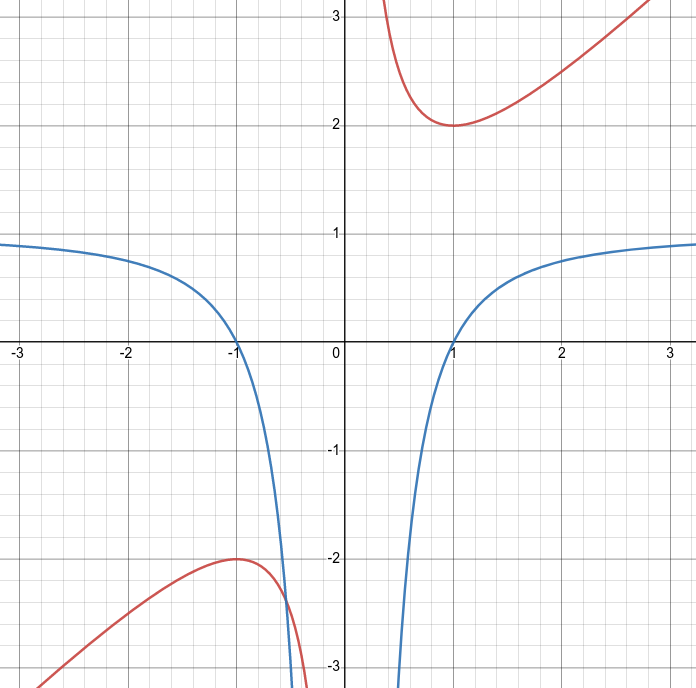
\includegraphics[scale=0.4]{fig_1.png}
		\caption{In red, graph of $f(x)$ and, in blue, the graph of $f'(x)$}
		\end{figure}
	\end{enumerate}
	
	\spc
	
	\exo{40}
	\\
	The function is not differentiable at $x = -1$ because $f$ is not continuous.
	
	The function is not differentiable at $x = 2$ because there is a corner in the graph of $f$ (the limit slope from the left and from the right are not the same).
	
	\spc
	
	\exo{48}
	\\
	We have to take a look at the slope of the tangent lines in each graph. 
	
	We can see that the curve ``c'' is positive where the slopes of the tangents to the graph of the curve ``d'' are postive. Also, we see that the curve ``c'' is negative when the slopes of the tangents to the graph of the curve ``d'' are negative. So the curve ``c'' represents the derivative of ``d''.
	
	We remark that the sign of the $y$-coordinate of the points of the curve ``b'' is the same as the slopes of the tangents to the curve ``c''. So curve ``b'' is the derivative of the curve ``c''. 
	
	Finally, we see that the sign of the slopes of the tangents to the curve ``b'' are always positive or zero and this is the same sign as the $y$-coordinate of the points on the curve ``a''. So the curve ``a'' is the derivative of the curve ``b''.
	
	In summary, we have
		\begin{align*}
		f \leftrightarrow d \text{, } f' \leftrightarrow c \text{, } f'' \leftrightarrow b \text{ and } f''' \leftrightarrow a .
		\end{align*}
	

\end{document}